\documentclass[12pt]{article}
\usepackage[fr, maths, tensoriel, matlab, natbib]{jd}
\usepackage{chngpage}

\geometry{hmargin=1.5cm, vmargin=1.5cm}

% small MATLAB listings
%\makeatletter
%\lst@AddToHook{TextStyle}{\let\lst@basicstyle\ttfamily\footnotesize\fontfamily{pcr}\selectfont}
%\makeatother
\lstset{basicstyle=\tiny\ttfamily}
\makeatletter
\def\thickhrulefill{\leavevmode \leaders \hrule height 1pt\hfill \kern \z@}
\def\blurb{%
  Université Paris 6 Pierre et Marie Curie \\
  M1 Océan, atmosphère, climat et télédétection \\[1em]}
\def\stage{Stage de M1}
\author{%
Jean-Denis Vauguet\\
\email{jd@typhon.org}}
\title{Caractérisation de l'effet lié aux vents et à la viscosité sur la propagation des ondes de gravité dans l'atmosphère}
\def\direction{%
{\Large Sous la direction de}\\[0.3em]
{\LARGE Giovanni \sc{Occhipinti}}\\[0.3em]
{\Large Équipe Études spatiales et planétologie -- IPGP}}
\date{2009}

\def\maketitle{%
  \null
  \thispagestyle{empty}%
  \vskip 1cm
  \begin{center}
    \normalfont \blurb
    \Large \stage
  \end{center}
  \ifhmode\par\fi
  \vskip 1cm
  \hbox to \hsize{\hfill
    \vrule height 2pt width.5\hsize
    \hfill}%
  \vskip 1cm
  \begin{center}
    \huge \strut \@title \par
  \end{center}
  %\par
  \vskip 0.8cm
  \hbox to \hsize{\hfill
    \vrule height 2pt width.5\hsize
    \hfill}%
  \vfil
  \begin{center}
  \normalfont\LARGE\@author\par
  \end{center}
  \vfil
  \begin{center}
  \direction
  \end{center}
  \par
  \null
  \cleardoublepage
  }
\makeatother

\begin{document}
\maketitle

\tableofcontents

\section{Présentation}

\subsection{Contexte du stage}

Ce stage a été effectué au sein de l’équipe \hyperref{http://ganymede.ipgp.jussieu.fr}{}{}{Études spatiales et planétologie} (IPGP UMR 7154 -- CNRS -- Université Paris 7) dirigée par Philippe Lognonné, sous la direction de Giovanni Occhipinti. Les travaux de l'équipe sont rattachées à la planétologie et à l'observation de la Terre, notamment pour caractériser les mécanismes de couplage enveloppes solides--océan--atmosphère. L'étude des planètes telluriques sous l'angle de la télédétection et de la géophysique interne sont au cœur de l'activité de recherche fondamentale, avec de nombreuses applications pour des missions spatiales et d'observation. Le présent stage s'insérait dans la large thématique des couplages terre interne--atmosphère, \emph{via} la caractérisation des perturbations atmosphériques transitoires associés aux évènements sismiques.

\subsection{Les ondes de gravité internes atmosphériques}

Le travail effectué lors de ce stage a été consacré une étude paramétrique des ondes de gravité internes (IGW, \emph{internal gravity waves}) atmosphériques, limitée à l'effet des vents et de la viscosité. Les IGW constituent la réponse à une perturbation d'un milieu fluide stratifié, généralement verticalement sous l'effet d'un champ de pesanteur et pour lequel la force d'Archimède joue le rôle de force de rappel — océan et atmosphère répondent en particulier à cette définition. Cette structuration verticale impose aux IGW une propagation tributaire de divers paramètres influençant, à différentes échelles, la stratification et donc le milieu de propagation des ondes, ainsi que les ondes elle-mêmes. On pourra ainsi avoir pour objectif de caractériser l'influence de phénomènes dissipatifs, d'interactions et de couplages, et ce dans les différentes couches atmosphériques.

Eu égard à leur rôle important dans l'évolution de la circulation et de la structure atmosphérique, notamment aux grandes échelles, les IGW constituent un sujet d'étude relativement récent. Dans une synthèse sur les travaux des deux dernières décennies, \cite{Fritts2003} insistent sur les progrès réalisés notamment grâce à l'avènement de la télédection et d'une modélisation numérique puissante : propagation verticale, phénomènes d'interactions et de turbulence, caractérisation spectrale…

Par conservation de l'énergie cinétique, la propagation des IGW atmosphériques donne lieu à une amplification — qui peut être très importante — proportionnelle à l'inverse de la racine carrée de la densité atmosphérique. Le phènomène se réalise sous contrainte du milieu local de propagation (atmosphère libre, ionisée, régime des vents, gradients de température, de vorticité, etc.) La propagation affecte le milieu de propagation, par exemple en générant de la turbulence et par dépôt d'énergie (phénomènes dissipatifs). D'un point de vue expérimental, la signature des IGW est plus particulièrement mise en évidence, par télédétection, à travers la perturbation qu'elle induit dans la très haute atmosphère ionisée (ionosphère) où se réalise un couplage magnétique. Cette perturbation dépend donc en partie des évènements ayant eu lieu lors de la propagation dans l'atmosphère neutre.

Le stage proposait de réaliser une étude de l'effet des vents et de la viscosité sur la propagation des IGW dans une atmosphère neutre réaliste (modèle \emph{U.S. Standard Atmosphere}, USSA76), indépendamment d'un couplage au champ magnétique terrestre dans l'atmosphère ionisée. Un travail analytique préparatoire devait mener à une implémentation numérique. Les IGW sont plus particulièrement au cœur de la « sismologie atmosphérique » qui vise à caractériser la signature atmosphérique des évènements sismiques, qu'ils aient été générés dans les structures internes ou dans l'enveloppe gazeuse. Plus particulièrement, il s'agissait ici de pouvoir caractériser des IGW tsunamigéniques intervenant dans le couplage sismique terre solide -- océan -- atmosphère. Une caractérisation fine de la propagation des ondes liées aux évènements sismiques océaniques est la clé pour la résolution de problèmes inverses et la prévention sismique.

%Du fait de la conservation de l’énergie cinétique et de la diminution de la densité atmosphérique en
%altitude (‫= ݇ܧ‬    ݉‫ ,)2ݒ‬l’atmosphère joue le rôle d’amplificateur naturel de la vitesse verticale (au sol)
                %ଵ
                %ଶ
                                                                %5
%qui est alors multipliée par un facteur pouvant aller jusqu’à 10 lorsque l’onde atteint l’ionosphère. Un
%des objectifs des nouveaux ‘sismologues atmosphériques’ est de pouvoir détecter cette onde via des
%satellites afin d’augmenter la densité des données sismiques et, dans le cas des tsunamis, de
%développer des nouveaux systèmes d’alertes préventives.


% TODO il faut parler de 1. milieu de propagation 2. milieu de détection avec des comportements et couplages différents dans les deux domaines atmosphériques

% nouvelle partie, sur la viscosité :

% copcol plus ou moins l'autre .tex, mais le réorganiser :
% petite intro/problématique (viscoisté négligeable d'aprèg Fritts…), puis
% ma dérivation analytique
% et ma tentative numérique, et pourquoi ça a foiré à mon avis

% en conclusion, ben… résumé plus ouverture sur ce que je vais continuer à faire


% --------------------------------------------------------------------------
%- pourquoi les étudier ?
%- quels sont les résultats généraux utiles ?
%- sur quels travaux précis se base mon travail (Sun…) ?
%- étude de l'effet des vents et de la viscosité : une partie analytique, une partie numérique
%- quels résultats ?
%- quelles perspectives ?


\section{Effets des vents}

\subsection{Modèle linéaire, phénomènes dissipatifs et filtre atmosphérique}

Les IGW représentent une solution des équations primitives atmosphériques (équation de Navier-Stokes \ie de la quantité de mouvement $\rho \vv$ pour un fluide newtonien) associées à des équations de conservation et/ou d'état bien choisies. Dans un modèle d'atmosphère réaliste, la masse volumique $\rho$ ne peut pas être considérée comme constante. Outre le champ de vitesse 3D $\vv$ et $\rho$, la pression $P$ apparaît évidemment comme cinquième inconnue. \cite{Occhipinti2008} proposent un système fermé basé sur les équations de continuité et de non-divergence, en l'absence de forçage :
\begin{subnumcases}{\label{eq:systeme}}
    \lp \delt{} + \vv \cdot \gradient \rp \vv &    $= -\frac{1}{\rho} \gradient P$    \label{eq:systeme-un} \\
    \divergence \vv &                      $= 0$                                                \label{eq:systeme-deux} \\
    \delt \rho + \divergence{\rho \vv} &   $= 0$                                                \label{eq:systeme-trois}
\end{subnumcases}

Ce modèle permet une étude directe de l'effet des vents. L'équation \refeq{eq:systeme-un} contient un terme advectif dont la complexité peut être réduite en considérant une approximation linéaire. Les ondes sont décrites comme la manifestation d'un (petit) écart à un état d'équilibre, dont la seule dépendance sera ici en $\textbf z$. On décompose ainsi $X \in \{ \vv = (u, v, w), \rho, \pression \}$ en la somme d'une partie moyenne $X_0(z)$ et d'une perturbation $X_1(x,y,z,t)$ (très petite devant la partie moyenne). Par ailleurs, sur la base d'une analyse en ordre de grandeur, on décide de négliger $\uzc$ devant $\uxc$ et $\uyc$. On applique l'approximation de Boussinesq (\ie $\rho_0$ partout sauf sur le terme de flottabilité, affecté de la perturbation — cela implique la non-divergence de la vitesse totale). Enfin, on linéarise au premier ordre en effectuant des développements limités sur $\rho$ au premier ordre (simplifiant les termes de pression et de gravité) et en ne prenant pas en compte les termes quadratiques et supérieurs ni les produits de perturbations. On cherche alors la solution de l'équation d'onde pour les cinq inconnues,  en prenant les transformées en ondes planes $X_1(x,y,z,t) = \tilde X(z) \cdot {\mathrm e^{i(\overbrace{k_x x + k_y y - \omega t}^{\textrm{phase~} \Phi})}}$. On obtient alors le système suivant dans le domaine spectral :
\begin{subnumcases}{\label{sys:S}(S)}
i \Omega \tux - \tuz \dz \uxc - \frac{1}{\rho_0} i k_x \tp = 0             \label{eq:igw-un}        \\
i \Omega \tuy - \tuz \dz \uyc - \frac{1}{\rho_0} i k_y \tp = 0             \label{eq:igw-deux}      \\
i \Omega \tuz - \frac{1}{\rho_0} \dz \tp - \frac{\trho}{\rho_0} g = 0      \label{eq:igw-trois}     \\
i k_x \tux + i k_y \tuy + \dz \tuz = 0                                     \label{eq:igw-quatre}    \\
i \Omega - \tuz \dz{\rho_0} = 0                                            \label{eq:igw-cinq}
\end{subnumcases}
avec $\Omega = \omega - \uxc k_x - \uyc k_y$ la fréquence intrinsèque liée au repère en mouvement.

Le fait de conserver des dérivées en $z$ en utilisant une phase spatialement 2D permet d'exprimer S sous la forme d'un propagateur du type $\dz V = A V$, avec :
\begin{align}
V & =
\begin{pmatrix}
    \tuz^* \\
    \tp^*
\end{pmatrix} \\
A & =
\begin{bmatrix}
    -\frac{1}{\Omega} \lp k_x \dz \uxc + k_y \dz \uyc \rp + \frac{1}{2} \dz{\ln{\rho_0}} & -\frac{i \lp k_x^2 + k_y^2 \rp}{\Omega}   \\
    i \lp \Omega + \frac{g}{\Omega} \dz{\ln{\rho_0}} \rp                                  & -\frac{1}{2} \dz{\ln{\rho_0}}             \notag
\end{bmatrix}
\end{align}
Les $*$ dénotent une renormalisation des deux paramètres $\tuz$ et $\tp$ : $\tuz^* = \sqrt{\rho_0} \tuz$ et $\tp^* = \frac{\tp}{\sqrt{\rho_0}}$ (d'où les termes en $\pm \frac{1}{2} \dz{\ln{\rho_0}}$). Cette renormalisation proportionnelle à la racine carrée de l'énergie assure que les perturbations de la vitesse verticale et de la pression sont indépendantes de l'amplification exponentielle avec $z$. Au final, le système ainsi construit permet une étude modale atemporelle pour ces deux inconnues, en fonction de l'état moyen de l'atmosphère (profils des vents, de densité, …) et du choix des paramètres spectraux, \ie périodes et longueurs d'onde.

Dans ces équations n'apparaissent pas explicitement de termes dissipatifs, lesquels seraient liés par exemple à de la dissipation thermique, des interactions d'ondes, du déferlement, ou bien de la diffusion de quantité de mouvement (viscosité). La théorie linéaire dérivée dans ces conditions se prête bien à une étude modale mono-paramétrique, mais il faut garder à l'esprit que les ordres de grandeur absolus déduits de simulations opérées sous ces conditions n'ont qu'une valeur limitée, car les mécanismes dissipatifs et les interactions multi-échelles sont vraisemblablement primordiaux dans les cas réalistes (\cite{Fritts2003}). Par ailleurs, en ne considérant ni les transferts au flux moyen, ni la turbulence induite, ni les échanges de chaleur, on ne s'autorise aucun \emph{feedback} lors de la propagation pseudo-spectrale. C'est donc avec un modèle « découplé » que le travail numérique a été effectué.

% copcol depuis l'autre .tex le système linéarisé, sans viscosité, le propagateur.
% parler des phénomènes dissipatifs en général, puis des deux paramètres étudiés : vent et viscosité
% pour le vent, en fait c'est pas toujours dissipatif ! étude de Sun et al, puis mon objectif : vérifier et étudier un cas « réaliste » d'un point de vue modal (filtre directionnel)

% nouvelle partie, sur les vents :
% dire comment on le passe en numérique, que j'ai fait une version vectorielle assez stable et rapide
% décrire les deux types d'instabilité : limite acoustique, ok, et explosion, qui elle fait référence à la partie suivante (préconditionnement)
% code en annexe, clean, décrire vite fait son fonctionnement
% donner des résultats parlant : un truc paramétrique, et un pour le modèle

Un double objectif a été poursuivi dans la paramétrisation par les vents moyens :
\begin{itemize}
    \item vérifier avec un modèle mono-paramétrique les résulats de \cite{Sun2007} qui, sur la base d'une analyse spectrale, estiment que les vents pourraient agir comme un filtre directionnel, permettant aux IGW se propageant contre le vent moyen d'atteindre plus rapidement et avec un minimum de perte énergétique la ionosphère ;
    \item examiner le rôle des vents moyens issus d'un modèle réaliste.
\end{itemize}

\subsection{Implémentation numérique}

En relation avec \cite{Occhipinti2008} existait un code de test MATLAB itératif, pour lequel les dimensions horizontales étaient réduites à une seule. Il servait à valider des calculs en amont d'une implémentation dans un code FORTRAN 3D entièrement spectral destiné à traiter des jeux de données massifs sur des architectures puissantes. L'étude de l'effet des vents à été menée sur la base du code MATLAB, transformé en un solveur vectoriel (\hyperref{annexe:A:modesTvectwind.m}{}{}{modesT-vect-wind.m}).

Le propagateur décrit ci-avant a été discrétisé par des différences finies centrées afin de fournir un système linéaire du type $KU~=~B$, avec $U$ le vecteur solution (contenant autant de couples $\lp \tuz^*~~\tp^* \rp$ que de pas de calculs), $B$ le vecteur second membre (identiquement nul, sauf pour les conditions initiales) et $K$ une matrice creuse de cœfficients issus du propagateur. Le couple de conditions initiales traduit la continuité de la perturbation de la vitesse verticale au sol (premier pas d'intégration), qui a été prise unitaire dans la perspective d'une étude modale prénormalisée. La pression initiale est déduite des caractéristiques spectrales imposées pour l'étude ($P_0 \propto (\omega, k_x, k_y, k_z)$ et $k_z \propto (k_x, k_y, N^2)$ où $N^2$ est la fréquence de Brunt–Väisälä).

En plus de la version vectorielle pseudo-3D (ondes sphériques), des scripts annexes (\hyperref{annexe:A:windeffect.m}{}{}{wind-effect.m}, \hyperref{annexe:A:dataprocessing.m}{}{}{data-processing.m}, \hyperref{annexe:A:mantexpnt.m}{}{}{mantexpnt.m}) ont été développés pour traiter les données (extraction, détection de la divergence, etc.) et produire des sorties graphiques synthétiques.

% TODO
% Le modèle d'atmosphère utilisé
% le modèle de vents
% dire que le code itératif avait deux types de divergence (acoustique, précision) et que le domaine de stabilité a été étendue pour la seconde avec le code vectoriel

\subsection{Résultats}

L'étude spectrale de \cite{Sun2007} repose également sur la théorie linéaire des IGW dans l'approximation des petites perturbations. Une fonction de transfert proche du propagateur présenté ci-avant est utilisée pour explorer les caractéristiques de la propagation atmosphérique, dans un modèle avec une composante visqueuse et des transferts de chaleur. De façon analogue, l'interface sol--atmosphère porte le signal d'entrée et les conditions initiales. Il est montré que, pour un modèle de vent moyen SE-NW (HWM93, \cite{Hedin1991}), les IGW dans la bande de période de 15 à 30 mn et de longueur d'onde de 200 à 400 km ont le plus de chance d'atteindre 300 km d'altitude, surtout si elles se propagent contre le vent moyen (\ie dans une direction NE-SW).

Les tsunamis sont associés à des périodes de l'ordre de quelques minutes à une heure, avec des longueurs d'ondes de 10 à 500 kilomètres. Compte tenu de la relation donnant la vitesse des ondes surfaciques induites, pour une hauteur moyenne océanique de 2500 km, on trouve que le domaine spectral dans lequel se réalise en première approximation le transfert d'énergie entre les ondes tsunamigéniques et les IGW correspond assez bien au domaine mis en évidence par Sun \emph{et al.} Toutefois, une large gamme de couples fréquence/nombre d'onde sont envisageables en raison des sources multiples d'IGW.

La figure \ref{fig:modes-scales} présente les résultats d'une simulation 2D sur trois fréquences, pour des IGW portant les caractéristiques spectrales d'une source tsunamigénique, associées à un gradient de vent linéaire fixé de 0 à $\pm$ 20 m.s$^{-1}$, et pour une gamme de trois longueurs d'onde initiales imposées par la relation entre nombre d'onde, période et vitesse de phase. On observe une augmentation de l'amplitude de la perturbation de la vitesse verticale avec un écrasement des modes, bien marqués après 125 km. Cette altitude correspond à la thermopause, à partir de laquelle a lieu un transfert énergétique entre les champs de pression, de densité et de vitesse horizontale d'une part, et le champ de vitesse verticale d'autre part. La thermosphère ainsi perturbée, et plus particulièrement la ionosphère, peut jouer le rôle d'amplificateur, un processus auquel se surimposera l'effet des vents. 

Le même type de simulation à basse résolution a été réalisé avec un modèle de vent NRLMSISE-00 (\cite{Picone2002}, figure \ref{fig:nrlmsise}). On observe (figure \ref{fig:modes-scales-picone}) une modulation des modes (en terme de valeur des maximums normalisés d'amplitude de la perturbation de vitesse verticale) en fonction du régime des vents moyens. Une comparaison des simulations avec vent zonal seul, vent méridional seul et le couple de vents montrerait que la composante de vent perpendiculaire à la direction de propagation des IGW n'a que peu d'influence sur celle-ci. Les vents contraires ont en effet tendance à écraser le paquet d'onde, et les vents portant à l'étaler, ce qui conduit respectivement à une diminution et une augmentation de la dissipation énergétique lors de la propagation, avec une dépendance à l'angle entre direction de propagation et direction du vent moyen. En l'absence de termes dissipatifs associés à la diffusion moléculaire et thermique, les variations d'amplitudes maximales affectent des gammes de périodes un peu plus élevées que pour Sun \emph{et al.}, mais l'observation principale est que l'intensité du gradient de vent est le facteur principal pour l'amplification dans le modèle mono-paramétrique, avant les caractéristiques fréquentielles de l'IGW soumise à ce gradient. Dans un cas réaliste, les phénomènes dissipatifs, outre leur effet additionnel de filtre spectral, entraveront l'amplification.

\begin{figure}[!ht]
\centering
\subfigure[]{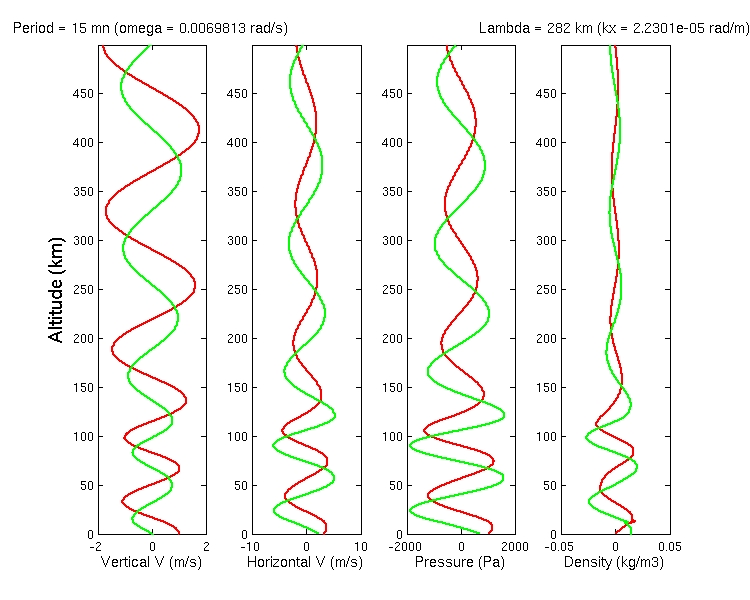
\includegraphics[width=0.45\linewidth]{01}}
\subfigure[]{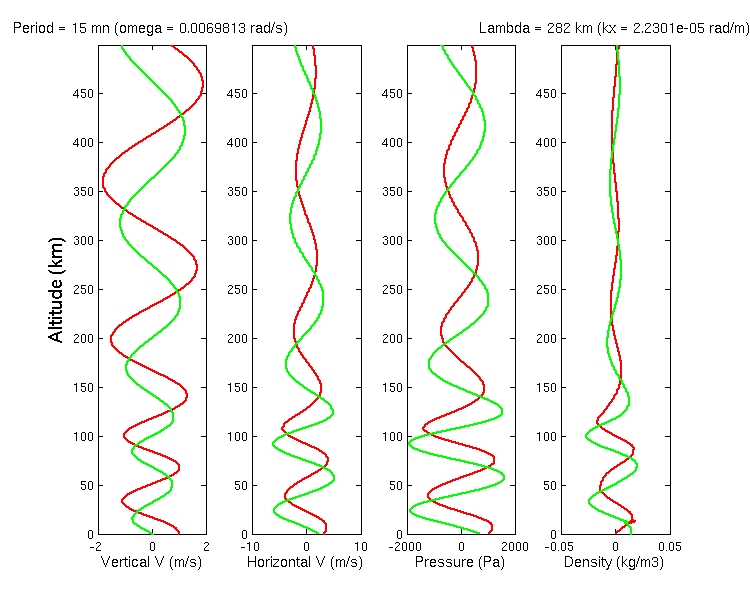
\includegraphics[width=0.45\linewidth]{03}}\\
\subfigure[]{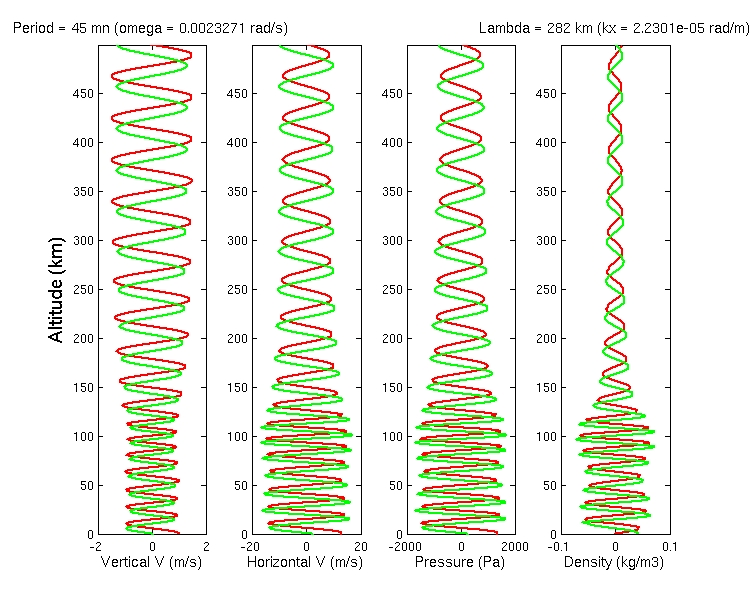
\includegraphics[width=0.45\linewidth]{02}}
\subfigure[]{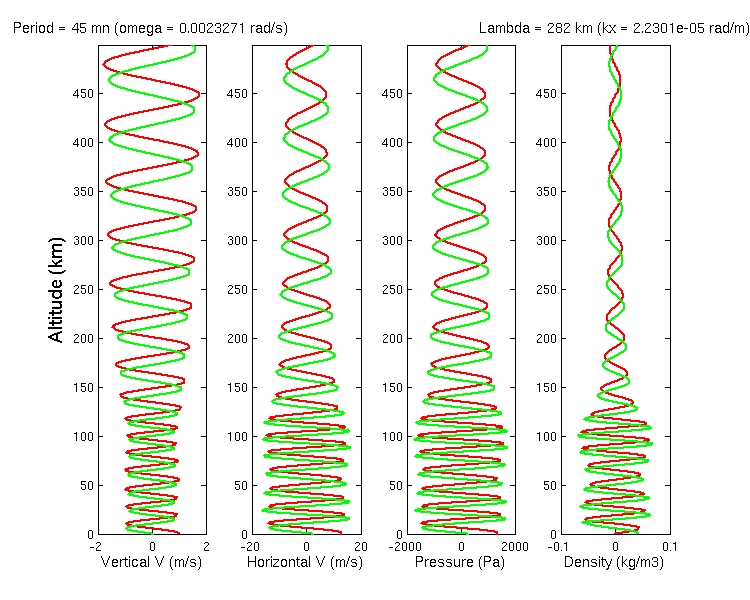
\includegraphics[width=0.45\linewidth]{04}}\\
\subfigure[]{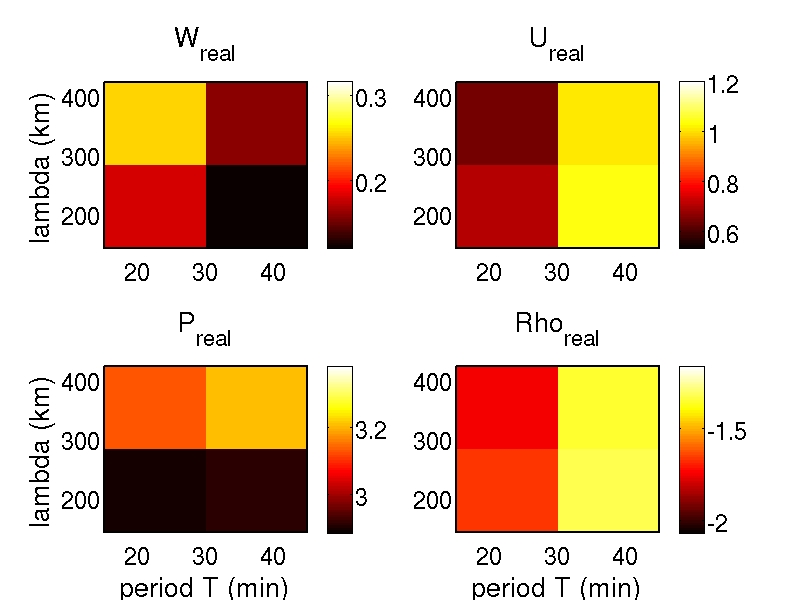
\includegraphics[width=0.45\linewidth]{05}}
\subfigure[]{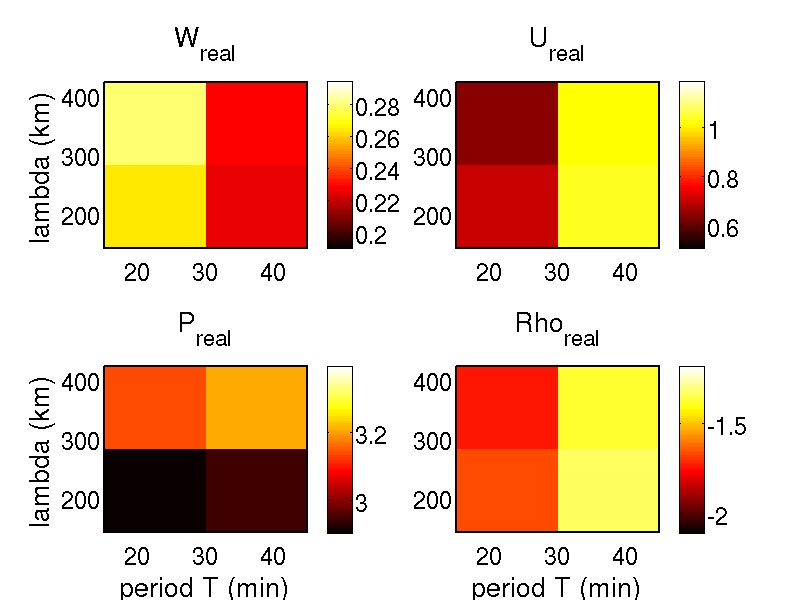
\includegraphics[width=0.45\linewidth]{06}}
\caption{Modes reliés à une onde tsunamigénique pour un gradient de vent linéaire de 0 à 20 m.s$^{-1}$ (a, c, e) et de 0 à -20 m.s$^{-1}$ (b, d, f). Périodes de 15 mn (a, b) et 45 mn (c, d). Maximum d'amplitudes respectifs dans l'espace des $k-\lambda$ (e, f).}
\label{fig:modes-scales}
\end{figure}

\clearpage
\changepage{3cm}%amount added to textheight
           {}%amount added to textwidth
           {}%amount added to evensidemargin
           {}%amount added to oddsidemargin
           {}%amount added to columnsep
           {-2cm}%amount added to topmargin
           {}%amount added to headheight
           {}%amount added to headsep
           {}%amount added to footskip
\begin{figure}[!ht]
\centering
\subfigure[]{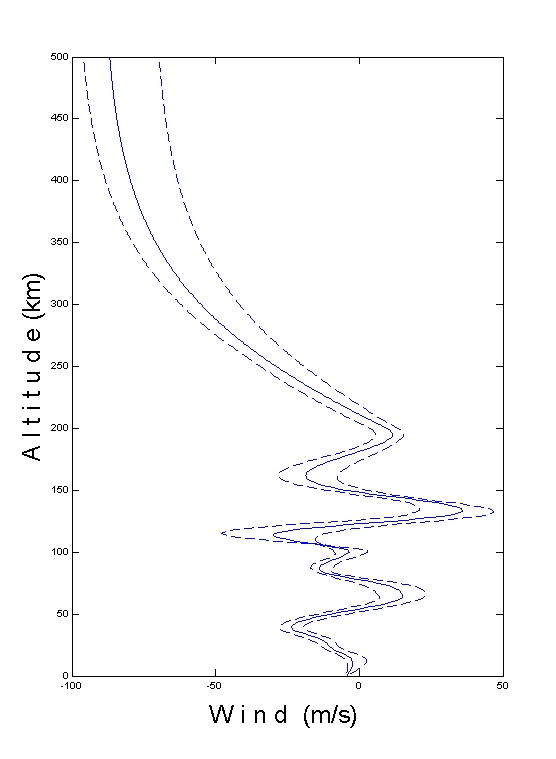
\includegraphics[width=0.3\linewidth]{Wind_Z}}
\subfigure[]{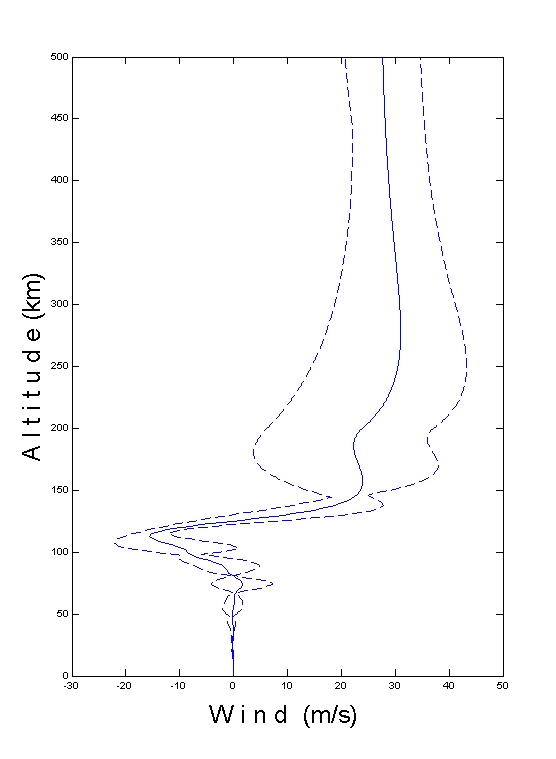
\includegraphics[width=0.3\linewidth]{Wind_M}}\\
\caption{Modèle de vent NRLMSISE-00 à 01H00 UT. Vent zonal (a) et vent méridien (b). Les courbes pleines sont les profils aux coordonnées géographiques [0°N; 85°E] (utilisés pour les simulations numériques), les lignes en pointillés montrent les variations des valeurs dans une grille de coordonnées [$\pm$12°N; (75°E,95°E)].
}
\label{fig:nrlmsise}
\end{figure}

\begin{figure}[!ht]
\centering
\subfigure[]{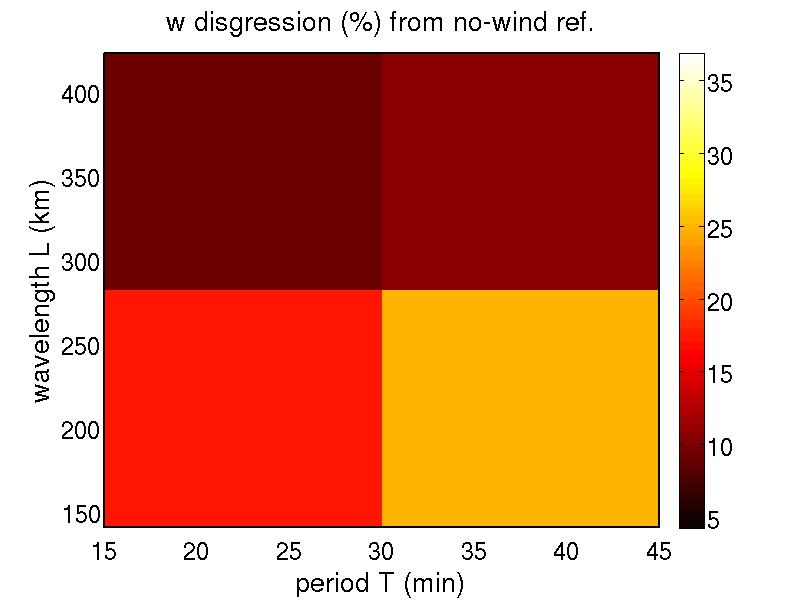
\includegraphics[width=0.4\linewidth]{disgression-w0-20T15+30+45Lauto}}
\subfigure[]{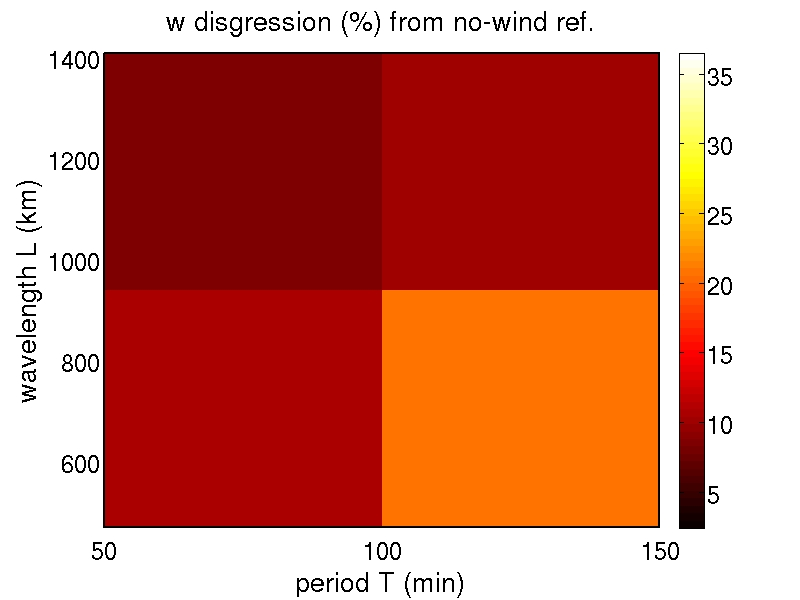
\includegraphics[width=0.4\linewidth]{disgression-w0-20T50+100+150Lauto}}\\
\subfigure[]{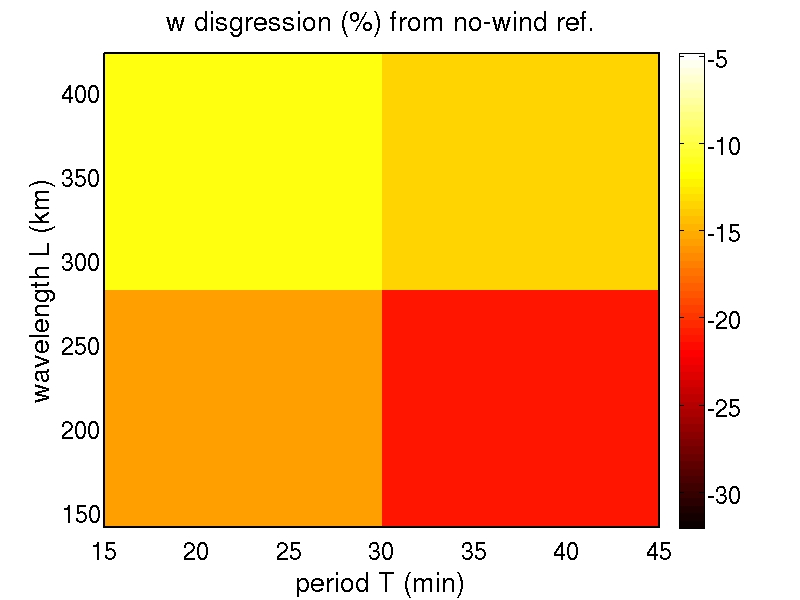
\includegraphics[width=0.4\linewidth]{disgression-w0+20T15+30+45Lauto}}
\subfigure[]{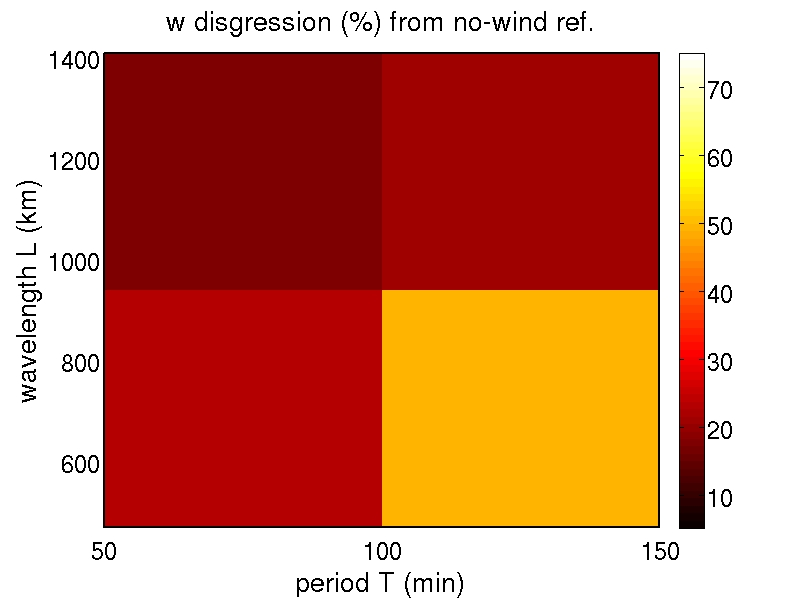
\includegraphics[width=0.4\linewidth]{disgression-w0-50T50+100+150Lauto}}
\caption{Écarts entre les maximums d'amplitude normalisés dans une atmosphère neutre pourvue d'un profil de vents moyens NRLMSISE-00 et les maximums normalisés pour une atmosphère neutre sans vents : pour un gradient de vent de 0 à -20 m.s$^{-1}$ pour deux gammes de fréquences (a, b), pour un gradient de vent de de 0 à +20 m.s$^{-1}$ (c), pour un gradient de vent de 0 à -50 m.s$^{-1}$ (d).}
\label{fig:modes-scales-picone}
\end{figure}
\vfill


\changepage{-3cm}%amount added to textheight
           {}%amount added to textwidth
           {}%amount added to evensidemargin
           {}%amount added to oddsidemargin
           {}%amount added to columnsep
           {2cm}%amount added to topmargin
           {}%amount added to headheight
           {}%amount added to headsep
           {}%amount added to footskip
\section{Modèle visqueux}

À l'échelle de la propagation des IGW, le milieu atmosphèrique possède une viscosité faible mais non négligeable sous certaines conditions rencontrées notamment dans la haute atmosphère. La diffusion de quantité de mouvement qui lui est associée peut constituer un phénomène dissipatif de premier plan des ondes amplifiées, au coté de la diffusion thermique et de la turbulence. Les IGW développées par des sources de basses/moyennes altitudes (topographie, cisaillement de vents, convection…) transportent de l'énergie et de la quantité de mouvement des régions de haute densité vers des régions de plus faible densité. L'estimation de l'efficacité de leur dissipation est essentielle pour paramétrer cette redistribution énergétique : des simulations numériques en ont dressées les caractéristiques principales (voir par exemple \cite{Vadas2005}).

Afin d'introduire sans \emph{a priori} ce nouveau paramètre dans le modèle utilisé pour l'étude modale, une revue du problème sous un angle rhéologique (\cite{Gueguen1994}) a tout d'abord été effectuée, en délaissant en première approche la dérivation usuelle mais complexe d'une relation de dispersion à dépendance fréquentielle. Une implémentation numérique de la propagation visqueuse dans une atmosphère neutre a ensuite été entreprise.

\subsection{Dérivation analytique}

En partant de la forme locale générale de l'équation de la dynamique
\beq \quad \rho \left ( \delt \vv + \vv \cdot \gradient \vv \right ) = \divergence \Tctr + \vf \quad \label{eq:dynamique} \eeq

avec $\vf$ la densité volumique des forces extérieures et $\Tctr$ le tenseur des contraintes. Par définition, $tr(\Tctr) = -\bar \pression \cdot$ dim, avec dim = 3 en 3D ($\bar \pression$ est la pression thermodynamique, identifiée à la pression hydrostatique $\pression$ pour la plupart des cas d'étude). De ce fait, on peut écrire \beq \Tctrij = \Tctrijdev - \kro \Tctrmoyij \eeq en séparant la partie déviatorique de la partie moyenne (isotrope).
\plop
Soit $\vu$ le vecteur déplacement, \emph{i.e.} $\vu = \overrightarrow{XX'}$ avec $X$ et $X'$ les positions d'un même point avant et après déformation. On définit le tenseur des déformations $\Tdef$ (\emph{strain tensor}) comme la partie symétrique de la matrice du gradient de déplacement \beq \Tdefij = \Tdefexpansion \eeq On a $tr(\Tdef) = \kro \Tdefij = \frac{\Delta V}{V} = \divergence \vu$, et on définit $\Tdefmoy = \frac{tr(\Tdef)}{3}$. Dès lors \beq \Tdefijdev = \Tdefij - \Tdefmoy \eeq

Soit $\vv$ le vecteur vitesse. On définit le tenseur du taux de déformation $\Ttxdef$ (\emph{strain rate tensor}) comme la partie symétrique de la matrice du gradient de vitesse, \emph{i.e.} la dérivée temporelle de $\Tdef$ \beq \Ttxdefij = \Ttxdefexpansion \eeq On a $tr(\Ttxdef) = \kro \Ttxdefij = \divergence \vv$ et on définit $\Ttxdefmoy = \frac{tr(\Ttxdef)}{3}$. Dès lors \beq \Ttxdefijdev = \Ttxdefij - \Ttxdefmoy \eeq
\plop
En utilisant la même idée de séparation entre une partie moyenne isotrope et une partie déviatorique, on peut exprimer toute la complexité du lien (tenseur d'ordre 4) entre contrainte et déformation dans le cas isotrope au moyen de deux cœfficients : un pour la variation de volume, un pour le cisaillement.

La viscosité newtonienne isotrope est définie telle que
\begin{subnumcases}{\label{eq:visc}}
    \Tctrijdev & $=\quad 2 \visc ~   \Ttxdefijdev$             \label{eq:visc-un} \\
    \Tctrmoy   & $=\quad ~ \viscbulk \divergence \vv$         \label{eq:visc-deux}
\end{subnumcases}
et l'élasticité isotrope est définie telle que
\begin{subnumcases}{\label{eq:elas}}
    \Tctrijdev & $=\quad 2 G ~ \Tdefijdev$                    \label{eq:elas-un}\\
    \Tctrmoy   & $=\quad ~ K ~ \divergence \vu = -\pression$  \label{eq:elas-deux}
\end{subnumcases}

où $\visc$ est la viscosité dynamique (aussi dite primaire, en cisaillement, \emph{shear viscosity}) et $\viscbulk$ la viscosité de volume (\emph{bulk viscosity}), en pascal seconde ; $G$ est le module de cisaillement, $K$ le module de compressibilité, en pascal.
%(note : $\viscbulk$ est notée $K$ dans le pdf en italien sur la viscosité que tu m'as donné).

Pour les fluides, qui se caractérisent par $G = 0$ (résistance nulle au cisaillement), un modèle classique consiste à prendre Kelvin%
\footnote{%
    Modèle de Kelvin type « ressort et amortisseur en parallèle » :
    \begin{numcases}{}
        \Tdef^{\textrm{élastique}}     & $=\quad \Tdef^{\textrm{visqueux}}$ \notag \\
        \Tctr                         & $=\quad \Tctr^{\textrm{élastique}} + \Tctr^{\textrm{visqueux}}$ \notag
    \end{numcases}
}
en volume ($\Tctrmoy$) et Maxwell%
\footnote{%
    Modèle de Maxwell type « ressort et amortisseur en série » :
    \begin{numcases}{}
        \Tctr^{\textrm{élastique}}     & $=\quad \Tctr^{\textrm{visqueux}}$ \notag \\
        \Ttxdef                     & $=\quad \Tdef^{\textrm{élastique}} + \Tdef^{\textrm{visqueux}}$ \notag
    \end{numcases}
} en cisaillement ($\Ttxdefdev$). Cela correspond à un comportement visco-élastique où la pression intègre toute la composante élastique. Si les forces volumiques dérivent d'un potentiel gravitationnel, \refeq{eq:dynamique} s'écrit
\begin{align}
\rho \dt{v_i}
  & = \deli{\Tctrij}{x_j} + \rho g_i \notag \\
\rho \dt \vv
  & = \divergence \Tctrdev + \divergence \overbrace{(- \pression + \viscbulk \divergence \vv)}^{\Tctrmoy} + \rho \vg \notag
  \intertext{et comme $G = 0$ pour les fluides, la partie déviatorique est purement visqueuse}
  & = \deli{2 \visc \Ttxdefijdev}{x_j} + \gradient \lp - \pression + \viscbulk \divergence \vv \rp + \rho \vg \notag \\
  \intertext{On montre que $2 \visc \divergence \Ttxdefdev = \visc \laplacien \vv$ (à $\visc$ constante, ce qui n'est pas irréaliste pour une application atmosphérique et facilite l'intégration numérique) et ce que l'hypothèse $\divergence \vv = 0$ soit appliquée ou non. De ce fait}
  \rho \dt{v_i} & = \visc \laplacien \vv + \gradient \lp - \pression + \viscbulk \divergence \vv \rp + \rho \vg \label{eq:dynamique-jd}
\end{align}

Par ailleurs, une expression du $\Tctrij$ visco-élastique \emph{pour les fluides newtoniens isotropes} est également donnée par une loi de comportement de Hooke mise sous la forme
\beq \Tctrij = - \kro \pression + \lambda \kro \Ttxdefkk + 2 \visc \Ttxdefij \eeq
où interviennent les cœfficients de Lamé : $\visc$ caractérise la résistance au cisaillement et $\lambda$ la compressiblité (constants pour un milieu homogène). On peut en déduire que la contrainte moyenne normale totale (viscosité + élasticité) vaut
\beq \Tctrmoy = \frac{\Tctrkk}{3} = -\pression + \left ( \lambda + \frac{2}{3} \visc \right ) \Ttxdefkk \eeq
donc \beq \viscbulk = \viscbulkexpansion \eeq
On peut dès lors utiliser cette formule pour calculer d'une autre manière le terme $\divergence \Tctrdev$ intervenant dans la forme locale \refeq{eq:dynamique}. On a
\begin{align}
\divergence \Tctrdev
  & = \lambda \gradient ( \divergence \vv) + 2 \visc \divergence \Ttxdef \notag \\
  & = \lambda \gradient ( \divergence \vv) + 2 \visc \divergence \left ( \Ttxdefdev + \Ttxdefmoy \right ) \notag \\
  & = \lambda \gradient ( \divergence \vv) + 2 \visc \divergence \Ttxdefdev + \frac{2\visc}{3} \gradient ( \divergence \vv ) \notag \\
  & = \underbrace{\lp \lambda + \frac{2\visc}{3} \rp}_{\viscbulk} \gradient ( \divergence \vv) + \visc \laplacien \vv \label{eq:dynamique-finale}
\end{align}
en cohérence avec \refeq{eq:dynamique-jd}.
  %; on peut éventuellement en déduire une forme rotationnelle}
  %& = \lambda \gradient ( \divergence \vv) + \visc \laplacien \vv - \visc \gradient ( \divergence \vv ) + \frac{5\visc}{3} \gradient ( \divergence \vv ) \notag \\
  %& = (\lambda + \frac{5\visc}{3} ) \gradient ( \divergence \vv) + \underbrace{\visc \laplacien \vv - \visc \gradient ( \divergence \vv )}_{- \visc \rotationnel(\rotationnel \vv)} \notag
Dans le cas d'un fluide de Stokes, on pose traditionnellement que $\viscbulk = \viscbulkexpansion = 0$.
%ce qui permet de simplifier l'expression ci-dessus en
%\beq (\lambda + \visc) \gradient ( \divergence \vv) - \visc \rotationnel(\rotationnel \vv) \label{eq:dynamique-lame} \eeq
Cette hypothèse n'est valide que pour les gazs monoatomiques et équivaut à poser que $\viscbulk = \frac{2 \visc(1 + \nu)}{3(1 - 2\nu)} = 0$ avec $\nu$ le cœfficient de Poisson, \ie $\nu = -1$ pour une viscosité primaire non nulle. Une telle valeur signifie que l'air est estimé être un milieu auxétique (le volume d'une parcelle réduit sous contrainte axiale par contraction dans la direction perpendiculaire à la contrainte). En réalité, l'air est un mélange gazeux. Toutefois, en appliquant à \refeq{eq:dynamique-jd} ou \refeq{eq:dynamique-finale} l'approximation de Boussinesq (impliquant $\divergence~\vv~=~0$), le terme en volume disparaît et on se ramène à la forme classique
\beq \rho \dt{\vv} = \visc \laplacien \vv - \gradient \pression + \rho \vg  \eeq

D'un point de vue numérique, conserver explicitement un terme en volume peut-être intéressant pour contrôler l'hypothèse $\divergence \vv = 0$ au regard des erreurs d'arrondis, en forçant sa nullité \emph{via} le champ de vitesse, si nécessaire. Physiquement parlant, cela revient toujours à poser que le travail des forces de viscosité est essentiellement lié au cisaillement ($\visc$), pas aux variations de volume (\emph{pas trop} de $\viscbulk$). Une limite $\nu = 0$ est atteinte (pas de variation de volume sous contrainte), auquel cas $\viscbulk = \frac{2\visc}{3}$. On conserve ainsi une composante visqueuse volumique isotrope en $\viscbulk \divergence \vv$, sous contrôle de $\divergence \vv = 0$.

%En terme de nombre de Deborah (\cite{Reiner1964}), rapport entre temps de relaxation de la perturbation et temps d'observation associé à l'échelle macroscopique la plus petite, le cas étudié se situe dans la limite $De = 0$. Elle correspond au cas newtonien, visqueux (faiblement, ici !), associé à un temps de relaxation de la perturbation nul, sous les hypothèses faites (Stokes + Boussinesq).

%\subsection{Réflexions et questions :)}

%%Déjà, à ce stade, j'ai noté que quand on décompose la contrainte entre la partie isotrope $\pression$ et la partie déviatorique (viscosité), on a beau dire qu'on a un fluide visqueux, en fait il est visco-élastique :) On a juste caché dans $\pression$ les contraintes résultantes de la pression/compression isotrope. Ça me semble ok du fait qu'on applique une approximation anélastique qui filtre les ondes de compression/dépression, mais souvent c'est vendu comme allant de soi dans les bouquins que j'ai pu lire. C'est assez trompeur…
%%\plop
%Un truc qui me gêne et avec lequel je n'arrive pas à m'accorder, compte-tenu de mes (faibles :)) connaissances actuelles. Annuler la viscosité de volume,
%\plop
%Dans mon esprit, si on suit un modèle « fluide de Stokes » mais sans le prendre au pied de la lettre, on cherche à dire que le travail des forces de viscosité est essentiellement lié au cisaillement (on mise sur $\visc$), pas aux variations de volume (on ne veut \emph{pas trop} de $\viscbulk$). C'est différent de dire que $\viscbulk = 0$ brutalement : ça signifie en fait qu'on vise une limite $\nu = 0$ (pas de variation de volume sous contrainte uniaxiale), auquel cas $\viscbulk = \frac{2\visc}{3}$ et on conserve une composante visqueuse volumique isotrope en $\viscbulk \divergence \vv$. Je ne suis personne pour remettre en question les approximations établies :) c'est juste que dans l'état de mes connaissances et en suivant « bêtement » mes calculs (que j'espère justes, mais…), quand je lis « $\viscbulk = 0$ définit le fluide de Stokes », j'arrive toujours à la conclusion que c'est bancal d'un point de vue physique (pas numérique…) et ce n'est pas le fait que $\viscbulk$ soit nul qui permet de négliger la viscosité de volume, mais la non-divergence sous l'approximation de Boussinesq (dans le cas présent). Dans le bouquin de Rieutord sur la dynamique des fluides, il est écrit : « en utilisant une approche statistique avec l'équation de Boltzman, on peut montrer que ce cœfficient [$\viscbulk$] est nul (du moins dans l'approximation de Boltzman) pour les gazs monoatomiques. Très souvent, on néglige purement et simplement $\viscbulk$ et lorsqu'on parle de la viscosité dynamique d'un fluide sans plus de précision, on entend $\visc$. Cette approximation qui consiste à négliger $\viscbulk$ s'appelle l'hypothèse de Stokes. On voit qu'en théorie elle ne convient bien qu'aux gazs monoatomiques. » Si tu as un avis sur la question, je suis preneur !
%\plop
%À partir de là, en me basant sur mes calculs rhéologiques :
%\begin{itemize}
%\item soit $\viscbulk \divergence \vv$ s'annule parce qu'on enchaîne sur l'approximation de Boussinesq qui impose $\divergence \vv = 0$, ce qui \emph{certes} revient analytiquement au même que d'avoir posé $\viscbulk = 0$ dès le début, mais à la mérite d'être cohérent avec un $\nu = 0$ plus « réaliste » qu'un cas auxétique (selon moi !) et évite de faire une hypothèse ou une autre sur la valeur de $\visc$ : ça n'impose que $\lambda = 0$, \emph{i.e.} l'incompressibilité. Ça à le mérite d'être assez cohérent ;
%\item soit on peut aussi conserver cette composante en $\divergence \vv$, car j'ai cru comprendre qu'en numérique, avoir $\divergence \vv = 0$ est une gageure, du fait des erreurs d'arrondis. Ça peut alors servir de critère pour surveiller la divergence du modèle (dixit Laëtitia Le Pourhiet ^^) : tant que le $\viscbulk \divergence \vv$ « visqueux » reste petit, on est bon. Sinon, il faut mettre en place un \emph{penality factor} pour corriger l'algorithme en cours de route (je ne sais pas faire là comme ça, mais ça a l'air marrant :)). \plop
%\end{itemize}

%Au final, voilà ce que j'en ai conclu avant de t'écrire ce petit document, pour te demander ton avis éclairé :
%\begin{itemize}
%\item on souhaite éliminer la composante de viscosité de volume $\viscbulk$ et ne conserver que la viscosité en cisaillement $\visc$ ;
%\item l'élasticité est en fait cachée dans la pression hydrostatique $P$, en cohérence avec…
%\item …l'approximation de Boussinesq qui filtre les ondes sonores (anélasticité) et qui permet de justifier mathématiquement pourquoi on en arrive de toute manière à négliger la viscosité en volume de façon élégante ;
%\item ça donne un fluide de Stokes au sens physique du terme, bien que je ne sois pas vraiment d'accord (mais ça vient peut-être de mon incompréhension totale du modèle !) avec l'assomption $\viscbulk = 0$ qui lui est associée dans la littérature (pour moi, ça donne un corps auxétique, bof). Par ailleurs, en faisant $\viscbulk = 0$, je ne trouve pas pareil que dans le texte sur la viscosité que tu m'as donné ($\frac{5}{3}$ au lieu de $\frac{4}{3}$), et je ne vois pas comment on peut trouver cette valeur sans choisir la valeur de $\lambda$, pas de $\viscbulk = \viscbulkexpansion$ ;
%\item à $\visc$ ($==$ en cisaillement) constante, il ne reste qu'un simple laplacien de la vitesse dans les équations — et comme on a les valeurs numériques de la viscosité en utilisant un modèle d'atmosphère (USSA76, NRLMSISE-00...), je crois comprendre que ça ne doit pas être gênant de poser nos calculs à $\visc$ constante, car les pas d'intégration sont petits devant l'échelle spatiale de variation de $\visc$. Utiliser la forme en laplacien me semble dès lors plus sympa que la forme en rotationnel du rotationnel et gradient de la divergence, non ?
%\item en terme de nombre de Deborah, on est au final dans une limite $De = 0$ qui correspond au cas uniquement visqueux, avec un temps de relaxation de la perturbation nul, sous les hypothèses faites (Stokes + Boussinesq).
%\end{itemize}

\subsection{Propagation visqueuse}

La réécriture du système S (\ref{sys:S}) en ajoutant la composante visqueuse sous la forme d'un laplacien du champ de vitesse fait apparaître une dérivée verticale seconde de $\vv$. Contrairement au cas non visqueux, dans lequel toutes les dérivées premières des composantes moyennes de la vitesse étaient advectées par une composante de la perturbation, cette dérivée seconde est « autonome. » En appliquant la même décomposition des $X \in \{ \vv = (u, v, w), \rho, \pression \}$ en la somme d'une partie équilibre $X_0(z)$ et d'une perturbation $X_1(x,y,z,t)$, le passage dans le domaine spectral injecte des facteurs $\neip$ pour ces termes du second ordre, ce qui traduit l'atténuation de la propagation moyenne sous l'effet dissipatif et qui affecte en retour l'évolution de la perturbation.
%Système de départ en se basant sur les calculs ci-avant :
%\begin{subnumcases}{\label{eq:systeme-IGW}(S)}
%\delt \vv + \vv \cdot \gradient \vv = - \frac{1}{\rho} \gradient \pression + \vect g + \nu \laplacien \vv \\
%\divergence \vv = 0 \\
%\delt \rho + \divergence{\rho \vv} = 0
%\end{subnumcases}
%\begin{subnumcases}{(S)}
%\delt \uxp + \uxc \delx \uxp + \uyc \dely \uxp + \uzp \delz \uxc =
%- \frac{1}{\rho_0} \delx \pp + \nu \left [ \left ( \delxs{} + \delys{} + \delzs{} \right ) \uxp + \dzs \uxc \right ] \notag \\
%\delt \uyp + \uxc \delx \uyp + \uyc \dely \uyp + \uzp \delz \uyc =
%- \frac{1}{\rho_0} \dely \pp + \nu \left [ \left ( \delxs{} + \delys{} + \delzs{} \right ) \uyp + \dzs \uyc \right ] \notag \\
%\delt \uzp + \uxc \delx \uzp + \uyc \dely \uzp =
%- \frac{1}{\rho_0} \delz \pp - \frac{\rho_1}{\rho_0} g + \nu \left [ \left ( \delxs{} + \delys{} + \delzs{} \right ) \uzp \right ] \notag \\
%\delx \uxp + \dely \uyp + \delz \uzp = 0 \hfill \notag \\
%\delt{\rho_1} + \uxc \delx{\rho_1} + \uyc \dely{\rho_1} + \uzp \delz{\rho_0} = 0 \notag
%\end{subnumcases}
%On cherche la solution de l'équation d'ondes en prenant $X_1(x,y,z,t) = \tilde X(z) {\mathrm e^{i(\overbrace{k_x x + k_y y - \omega t}^{\Phi})}}$ :
%\begin{subnumcases}{(S)}
%- i \omega \tux + \uxc i k_x \tux + \uyc i k_y \tux + \tuz \dz \uxc = - \frac{1}{\rho_0} i k_x \tp + \nu \left [ \left ( - k_x^2 - k_y^2 \right ) \tux + \dzs \tux + \neip \dzs \uxc \right ] \label{eq:igw-un} \\
%- i \omega \tuy + \uxc i k_x \tuy + \uyc i k_y \tuy + \tuz \dz \uyc = - \frac{1}{\rho_0} i k_y \tp + \nu \left [ \left ( - k_x^2 - k_y^2 \right ) \tux + \dzs \tuy + \neip \dzs \uyc \right ] \label{eq:igw-deux} \\
%- i \omega \tuz + \uxc i k_x \tuz + \uyc i k_y \tuz = - \frac{1}{\rho_0} \dz \tp - \frac{\trho}{\rho_0} g + \nu \left [ \left ( - k_x^2 - k_y^2 \right ) \tuz + \dzs \tuz \right ] \label{eq:igw-trois} \\
%i k_x \tux + i k_y \tuy + \dz \tuz = 0 \label{eq:igw-quatre} \\
%- i \omega \trho + \uxc i k_x \trho + \uyc i k_y \trho + \tuz \dz{\rho_0} = 0 \label{eq:igw-cinq}
%\end{subnumcases}
\begin{subnumcases}{(S)}
i \Omega \tux - \tuz \dz \uxc - \frac{1}{\rho_0} i k_x \tp + \nu \left [ \left ( - k_x^2 - k_y^2 \right ) \tux + \dzs \tux + \neip \dzs \uxc \right ] = 0   \label{eq:igw-un}       \\
i \Omega \tuy - \tuz \dz \uyc - \frac{1}{\rho_0} i k_y \tp + \nu \left [ \left ( - k_x^2 - k_y^2 \right ) \tux + \dzs \tuy + \neip \dzs \uyc \right ] = 0   \label{eq:igw-deux}     \\
i \Omega \tuz - \frac{1}{\rho_0} \dz \tp - \frac{\trho}{\rho_0} g + \nu \left [ \left ( - k_x^2 - k_y^2 \right ) \tuz + \dzs \tuz \right ] = 0              \label{eq:igw-trois}    \\
i k_x \tux + i k_y \tuy + \dz \tuz = 0                                                                                                                      \label{eq:igw-quatre} \\
- i \omega \trho + \uxc i k_x \trho + \uyc i k_y \trho + \tuz \dz{\rho_0} = 0                                                                               \label{eq:igw-cinq}
\end{subnumcases}
avec toujours $\Omega = \omega - \uxc k_x - \uyc k_y$.\\

Avant l'introduction de la viscosité, le propagateur dérivé du système était de la forme $\dz V = A V$. Obtenir une expression similaire n'est plus possible en raison de la présence des termes du second ordre. Il est par contre possible d'écrire un propagateur composite, somme d'un propagateur du premier ordre et d'un propagateur du second ordre dépendant du précédent. Numériquement parlant, l'approche immédiate (cf. \hyperref{annexe:B}{}{}{annexe B}) consiste à appliquer la méthode de résolution présentée pour l'effet des vents, en recalculant les composantes de $K$ et les seconds membres. Le champ de la perturbation de vitesse horizontale apparaît comme inconnue explicite dans les formulation des variables normalisées $\tuz^*$ et $\tp^*$ et doit donc être ajoutée au vecteur solution $U$, ce qui multiplie par deux la dimension du système en 3D. Des différences finies centrées d'ordre 2 sont introduites, si bien que les conditions initiales sont maintenant doublées afin d'initier la résolution au second ordre par une propagation non visqueuse.
Les calculs peuvent être effectués à $\visc$ constante tant que les pas d'intégration sont petits devant l'échelle spatiale de variation de $\visc$.

Cette méthode directe échoue car le système diverge très rapidement. La raison est en que certaines composantes de $K$ et de $B$ sont très proches de 0 au regard de la précision numérique disponible, de sorte que le système est fortement mal conditionné, avec notamment $K$ proche d'une matrice singulière (à déterminant nulle, \ie. non inversible).

Pour augmenter le taux de convergence vers une solution correcte, deux approches sont possibles :
\begin{itemize}
    \item au niveau de la dérivation analytique, adimensionner S en définissant des échelles caractéristiques pour les variables indépendantes et dépendantes.
    \item au niveau de la discrétisation, préconditionner $K$, afin de lui conférer des propriétés « spectrales » plus favorables à une résolution vectorielle. On souhaite alors se donner un préconditionneur $G$ qui, appliqué au système linéaire, permette de le ramener dans un domaine numériquement acceptable. Cette approche peut être utilisé en complément de l'adimensionnement, car le traitement spectral du système modifie les ordres de grandeurs.
\end{itemize}

À l'issue du stage, l'implémentation d'un code fonctionnel basé sur le système adimensionné n'était pas terminée, aussi l'étude numérique de l'effet de la viscosité n'a pas été menée à son terme. Toutefois, des considérations analytiques et numériques sont présentées ci-après.
%En fait, compte-tenu du pas spatial et du modèle atmosphérique utilisé, la dissipation visqueuse est attendue non négligeable à partir d'une hauteur de plusieurs dizaines de kilomètres. Pour le vérifier, on aurait pu implémenter une construction de $K$ en deux parties, en laissant le choix du seuil en altitude à partir duquel la propagation visqueuse prend le relais du cas non visqueux, et plotter l'écart relatif au cas non visqueux en fonction de z.

%Dans l'équation \refeq{eq:igw-quatre}, on isole le $\dz \tuz$ et on exprime les autres termes avec \refeq{eq:igw-un} et \refeq{eq:igw-deux} (on peut noter $\Omega = \omega - \uxc k_x - \uyc k_y$). Ça donne un des deux termes de V. Désormais, il y a dans le membre de droite des trois premières équations du $\dzs \tui$. Avec \refeq{eq:igw-trois} et \refeq{eq:igw-cinq}, on construit $\dz \tp$ en fonction de $\dz \tuz$.
%\plop
%Dans l'idée, le système linéaire se résout pareil que dans le cas non-visqueux, en différences finies. Je pense qu'il est sage de les calculer centrées, aux deux ordres, mais faut voir pour les conditions initiales. \emph{Todo asap} :)

\subsection{Adimensionnement, potentiel dissipatif de la viscosité}

% TODO
% partie précédente : décrire le raccordement sqrt(gh) !
% justifier l'échelle de longueur verticale !
% écrire le système adimensionné
% parler de la loi de similitude, Reynolds
% faire l'analyse en ordre de grandeur
% conclusion : le code visqueux ne le sera que partiellement, pour gain d'efficacité

Afin de réaliser l'adimensionnement du système étudié, il est nécessaire d'introduire des échelles typiques de temps (dynamique) et de longueur pour les variables indépendantes, de vitesse, de pression et de densité pour les variables dépendantes. Dans le cadre d'une étude modale, le choix de ces échelles est guidé par les caractéristiques spectrales du système. Une échelle typique de temps sera déduite de la période étudiée ; lui sera couplée l'échelle typique de longueur horizontale \emph{via} la longueur d'onde étudiée (choisie ou imposée par le raccordement IGW tsunamigénique -- IGW atmosphérique). On considèrera donc les paramètres en entrée du système (au sol). L'échelle typique de longueur verticale est moins contrainte (du fait de la forme explicite en $\tuz^*$) ; on la prendra égale à l'échelle horizontale pour des raisons numériques. Les échelles typiques de vitesses seront celles des vitesses au sol. Ainsi :
\begin{align}
u    & = U u^*, v = V v^*, w = W w^* \textrm{~avec~} U = V = W \\ \notag
x    & = L x^*, y = L y^*, z = L z^* \\ \notag
t    & = \frac{L}{U} t^*, P = \rho U^2 P^*, \rho = R \rho^* \notag
\end{align}
\begin{subnumcases}{(S)}
    \deltet{\vv^*} + \lp \vv^* \cdot \gradient \rp \vv^* & $= -\gradient P^* + \frac{\mu}{\rho U L} \laplacien \vv^*$ \\
    \divergence \vv^* & $= 0$ \\
    \deltet{\rho^*} + \divergence \lp \rho^* \vv^* \rp & $= 0$
\end{subnumcases}

On isole ainsi le nombre de Reynolds $Re = \Reynolds$ qui demeure le seul paramètre des équations du mouvements. En prenant 100 km comme ordre de grandeur moyen de la longueur d'onde et 1 pour la masse volumique, on a $Re = 10^{10}U$. Alors $Re \leq 1 \equivaut U \leq 10^{-10}$ ; on peut donc s'attendre \emph{a priori} à ce que la dissipation visqueuse soit négligeable. Toutefois, le profil de densité atmosphérique entre en jeu. Au sol, $\rho$ est de l'ordre de l'unité. Par exemple, vers 130 km d'altitude, le modèle USSA76 donne une valeur de $10^{-9}~\textrm{kg}.\textrm{m}^{-3}$, ce qui correspond à $Re = 10U$ \ie $U \leq 0,1~\textrm{m}.\textrm{s}^{-1}$. À partir d'une certaine altitude, selon l'ordre de grandeur des perturbations, il est attendu que la viscosité joue un rôle dissipatif non négligeable.

\subsection{Approche numérique}

Même adimensionné, un système n'est pas nécessairement conditionné de façon optimale. Dans le cas présent, le passage dans l'espace fréquentiel introduit des combinaisons de cœfficients de faible ordre de grandeurs. Un préconditionnement numérique peut être utile pour construire une méthode de résolution stable et extensible à d'autres paramètres (auquel cas l'adimensionnement analytique devient plus délicat).

Le principe général d'un préconditionnement pour un système linéaire $KU = B$ est de trouver $G$, approximation de $K^{-1}$, de sorte que $GKU = GB$ soit un système linéaire équivalent, à la précision numérique près, au système de départ. Évidemment, $G$ doit pouvoir être construit et appliqué rapidement. Si $G$ est une approximation directe de $A^{-1}$, le préconditionnement est explicite ; si $G = M^{-1}$ avec $M$ une approximation creuse de $A$, le préconditionnement est implicite et son application nécessite la résolution de systèmes linéaires dérivés.
%Déterminer $G$ n'est pas trivial et on peut-être amené à utiliser une des deux approches classiques : un préconditionneur itératif, basé sur un algorithmé généraliste « tout terrain » efficace mais non optimal, ou un préconditionneur ponctuel, déduit des propriétés spécifiques du système (symétrie, densité et magnitudes des valeurs, etc.) La seconde approche peut se révéler plus efficace, surtout s'il est possible de partir d'un algorithme itératif puissant, mais c'est un travail complexe.

Dans le problème étudié, les propriétes de $K$ amènent à penser qu'un préconditionnement explicite serait plus judicieux, car $K$ n'est pas symétrique : la plupart des méthodes de préconditionnement classiques, implicites, ne peuvent s'appliquer qu'à des matrices symétriques définies positives (SPD pour \emph{symmetric positive definite}) \ie symétrique et dont toutes les valeurs propres sont strictement positives. Par ailleurs, dans la perspective d'une parallélisation du code, l'application explicite présente une meilleure atomicité et réduit les besoins de communications. Les problèmes de convection-diffusion en particulier génèrent des systèmes linéaires fortement creux et non symétriques (NSPD) ; toutefois, des méthodes implicites plus généralistes, rapides, ont été récemment développées pour gérer les systèmes non symétriques (\cite{Rezghi2006}, \cite{Benzi1998}).

$K$ est en effet une matrice fortement creuse : un préconditionneur explicite efficace $G$ devrait dans l'idéal l'être dans les mêmes proportions. Sous ces conditions et en utilisant une méthode bien choisie, par exemple du type gradient conjugé, l'application de G au système pourra se limiter à de simples multiplications matrices-vecteurs. Toutefois, une approximation directe de $K^{-1}$ n'est pas nécessairement plus efficace qu'une approximation indirecte, car $K$ présente un caractère fortement diagonal qui se prête particulièreme bien à l'application des méthodes implicites, du type factorisation LU. Somme toute, les deux approches semblent judicieuses.



\section{Élements de conclusion}

\subsection{Résumé}
Une double étude mono-paramétrique modale des IGW atmosphériques a été menée, dans la perspective d'obtenir un code de simulation numérique où les différents paramètres importants pour la propagation 3D seraient intégrés. Au cours de ce stage, l'effet des vents et de la viscosité a été abordé. Le rôle des vents moyens comme filtre directionnel a été reproduit, en accord avec \cite{Sun2007} ; l'effet d'amplification/atténuation relative a par la suité été appliqué à un système d'IGW tsunamigénique, associé à un profil réaliste des vents atmosphériques. Une amplification importante est attendue pour les IGW se propageant contre le vent moyen.
% TODO donner le résultat essentiel pour le cas réaliste : qui quoi comment ?
Le rôle de la viscosité a été exploré analytiquement et les bases numériques ont posées, quoique l'implémentation effective n'est pas été achevée. L'adimensionnement du système d'étude s'est révélé nécessaire pour à terme intégrer numériquement les ordres de grandeur des différentes inconnues du problème.

\subsection{Bilan personnel du stage}

Je souhaite tout d'abord remercier Giovanni Occhipinti. Après avoir défini les objectifs généraux à atteindre, il m'a laissé toute latitude pour me familiariser avec mon sujet et l'aborder d'une manière ouverte. Nous avons peu communiqué et j'ai réalisé un travail indépendant -- sûrement trop ! Cette méthodologie présente des risques évidents de découragement et d'égarement, en partie expérimentés ; en contre-partie, cela m'a amené à prendre à bras le corps un sujet transverse et à réaliser un travail le plus cohérent possible. J'ai progressé analytiquement (en explorant les aspects rhéologiques pour contrôler un résultat qui me semblait douteux, et en envisageant — malheureusement un peu tard — l'adimensionnement de mon système d'étude) ; j'ai progressé numériquement (avec le soucis de faire un code vectoriel efficace, ce qui a été plus payant quoique les simulations aient été effectuées à basse résolution !).

Des notions importantes m'ont manqué en cours de route et je n'ai pas toujours, à tort, cherché de l'aide auprès de mon tuteur, souhaitant me « débrouiller » autant que possible par moi-même — erreur ! Le fait de travailler sur deux paramètres m'a amené progressivement délaisser l'un au profit de l'autre, \ie à privilégier le numérique sur l'analytique. Ayant gagné une meilleure compréhension des aspects adimensionnels dans les derniers jours du stage, la perspective d'achever l'étude et de continuer au-delà est réjouissante. Il s'agissait de ma toute première année universitaire en physique et ma motivation s'est trouvée renforcée par ce stage.

Évidemment, « coder » en amont du traitement de résultats est une tâche relativement solitaire et propice au surplace (bugs, nécessité d'apprendre en cours de route des techniques numériques spécifiques, donc de s'informer, produire les tests en relation, etc.) Je souhaiterais par la suite développer un code adimensionnel efficace, dans lequel il sera possible d'intégrer des paramètres supplémentaires. Il y aura alors la perspective de sortir de l'étude purement modale pour passer à un traitement basé, par exemple, sur les relations de dispersion. On pourra alors envisager de traiter des données réelles (Sumatra-Andaman, problème inverse), de paralléliser le code, etc.



\bibliographystyle{agu}
\bibliography{jd.bib}

\section{Annexes}

\subsection{A : codes pour l'étude modale de l'effet des vents}
\label{annexe:A}

\subsubsection{modesT-vect-wind.m}
\label{annexe:A:modesTvectwind.m}
code de résolution spectrale principal
\lstinputlisting{../../MATLAB/vectorial/3D/modesT_vect_wind.m}

\subsubsection{wind-effect.m}
\label{annexe:A:windeffect.m}
interface utilisateur pour une étude d'un profil de vent donné
\lstinputlisting{../../MATLAB/vectorial/3D/wind_effect.m}

\subsubsection{data-processing.m}
\label{annexe:A:dataprocessing.m}
utilitaire d'extraction des données
\lstinputlisting{../../MATLAB/vectorial/3D/data_processing.m}

\subsubsection{utilitaire mantisse/exposant}
\label{annexe:A:mantexpnt.m}
\lstinputlisting{../../MATLAB/vectorial/3D/mantexpnt.m}

\subsection{B : code visqueux}
\label{annexe:B}

code préparé pour la résolution d'un système adimensionné (et éventuellement préconditionné) -- pourra servir de base à une étude multiparamétriques (vents, viscosité, chaleur, etc.)
\lstinputlisting{../../MATLAB/viscovectorial/tmp.m}



\end{document}

